% Metódy inžinierskej práce

\documentclass[10pt,twoside,slovak,a4paper]{article}

\usepackage[slovak]{babel}
%\usepackage[T1]{fontenc}
\usepackage[IL2]{fontenc} % lepšia sadzba písmena Ľ než v T1
\usepackage[utf8]{inputenc}
\usepackage{graphicx}
\usepackage{url} % príkaz \url na formátovanie URL
\usepackage{hyperref} % odkazy v texte budú aktívne (pri niektorých triedach dokumentov spôsobuje posun textu)

\usepackage{cite}
%\usepackage{times}

\pagestyle{headings}

\title{Porovnanie metód modelovania webových aplikácií\thanks{Semestrálny projekt v predmete Metódy inžinierskej práce, ak. rok 2021/22, vedenie: Vladimír Mlynarovič}} 

\author{Patrik Tomčo\\[2pt]
	{\small Slovenská technická univerzita v Bratislave}\\
	{\small Fakulta informatiky a informačných technológií}\\
	{\small \texttt{xtomco@stuba.sk}}
	}

\date{\small 6. novembra 2021} 



\begin{document}

\maketitle

\begin{abstract}
%\ldots
Modely a modelovacie nástroje sú veľmi často používané softvérovými inžiniermi na vyjadrenie ich myšlienok počas vývoja softvéru. Tieto modely vedú k definícii modelovo-založeného vývojového procesu (MDD: Model-Driven Developement). Počas celej histórie softvérového inžinierstva boli pridávané nové využitia pre modely. Potenciálne benefity využívania modelov sú výrazne väčšie v softvérovej, ako v inej inžinierskej disciplíne.\cite{Selic:Pragmatics}. V MDE (Model-Driven Engineering) sú modely považované za hlavný vývojový artefakt na tvorbu softvéru. \cite{Gottardi:Metamodels}\\
Z toho môžme vyvodiť, že dôležitosť modelov v MDD je neodmysliteľná a je dôležité vedieť s nimi patrične narábať. 
Tento článok sa zaoberá popisom a porovnaním MDD metód, ktoré su esenciálne pre správne a dlhodobé fungovanie softvéru, ako aj pre jeho komplexnosť.
Taktiež analyzuje techniky navrhované na špecifikovanie funkčných, dátových a navigačných požiadaviek, ako aj poskytnutých mechanizmov na automatické preloženie týchto požiadaviek do koncepčných modelov. Hlavným cieľom tohto článku je preto pohľad a tieto metódy, využívaných vo vývoji webových aplikácií za účelom poukázania na ich silné a slabé stránky.\cite{Valderas:MDDE}\\
\\
Kľúčové slová: koncepčný model, modelmi riadený vývoj, metódy, webová aplikácia, modelmi riadené webové inžinierstvo, softvér
\\
\\ 
%Čo pokladáte za významný problém v tejto oblasti a prečo (opora v literatúre)?\\


\end{abstract}


\section{Úvod}

Modelmi riadený vývoj (MDD: Model-Driven Developement) sa stáva stále viac a viac dôležitou a využívanou metódou vrámci softvérového inžinierstva. 
MDD tvrdí, že softvérové systémy musia byť vyvíjané pomocou modelov. MDD proces zvyčajne začína požiadavkovou fázou, v ktorej sa definujú požiadavkové modely, z ktorých následne vzikne jeden alebo viacero koncepčných modelov~\ref{KM}. Tie majú za úlohu popísať systém bez prihliadnutia na technologické aspekty softvéru a sú neskôr využité v analytickej fáze\cite{Valderas:MDDE}. Práve týmto modelom a metódam, v ktorých su obsiahnuté,  je venovaný tento článok. Presnejšie porovnaniu jednotlivých metód a koncepčných metód z nich pozostavujúcich. Tento článok sa zaoberá popísaním rôznych MDWE (Model-Driven Web Engineering) metód. Tieto metódy a koncepčné modely článok porovnáva z pohľadu MDD, ako aj z pohľdaju funkcionality a navigácie v rámci webových aplikácií a požiadaviek používateľa na spomenutých stránkach. V dnešnej dobe existuje enormné množstvo metód zaoberajúcich sa vývojom webových aplikácií. Preto by si popísanie všetkých metód dopodrobna vyžadovalo príliš veľké úsilie. Tento čánok sa preto venuje len redukovanej množine metód, aby bolo možné sa im viac dopodrobna venovať. Metódy, ktorým sa článok primárne venuje sú OOHDM(Obejct-Oriented Hypermedia Design Model), OOWS(Object Oriented Web Solutions) a WSDM(Web Site Design Method). Každá z týchto metód predstavuje koncepčné modely, ktoré nám umožnujú popísať webové aplikácie technologicky nezávislým spôsobom. "Tieto metódy boli úspešne aplikované vo vývoji viacerých webových aplikácií, čo je dôkazom toho, že implementácia konštruovania webových aplikácií pomocou koncepčných modelov a ich neskoršie prepísanie do kódu je možné".\cite{Valderas:MDDE}\\

Pre porozumenie tejto problematiky je veľmi dôležité vedieť, čo presne koncepčné modely predstavujú. Preto tento článok začne ich popisom. Ďalej bude pokračovať následovne. Sekcia 3 prezentuje prehľad popisovaných MDWE metód a ich bližší popis. Sekcia 4 sa venuje porovaniu týchto metód a koncepčným modelom z pohľadu MDD a funkcionality a navigácie v rámci  webových aplkácií. Sekcia 5 sa podrobnejšie venuje popisu MDA (Model-Driven Architecture) prístupu, ktorý je neskôr využitý v následujúcej sekcii. Sekcia 6 je venovaná porovnávaniu metód a modelov využivajúcich spomenutý MDA prístup. Sekcia 7 slúži ako sumarizácia všetkého, čo sme zistili o danej problematike a posledná sekcia poskytuje prehľad bibliografie.\\
\\
Ešte spomeniem MDA prístup
\\
\section{Koncepčné modely} \label{KM}

Ako bolo spomenuté, táto sekcia sa venuje definícii koncepčných modelov. Pre spávne porozumenie neskoršej problematiky je znalosť týchto modelov veľmi dôležitá.\\
Koncepčné modely webových aplikácií špecifikujú jej kompozíciu a navigáciu v nej\cite{Gkatouna:Patterns}. Kompozícia web stránky definuje, ktoré stránky tvoria hypertext a ich internú kompozíciu, ako aj možnosti používateľa na zaobchádzanie so systémom. Navigácia definuje rôzne spôsoby, ako môžu byť dané stránky navzájom prepojené linkami, ale aj zobrazenie postupnosti stránok, na základe používania zo strany používateľa, a obsahom vyobrazeným na stránke. Inými slovami, koncepčné modely webových aplikácií špecifikujú organizáciu jej front-end rozhrania v podobe stránok, dizajnových elementov, ktoré sú prepojené linkami na uľahčenie navigácie na web stránke a manipulovania s ňou\cite{Gkatouna:Patterns}.
\\
\\
Možno ešte niečo napíšem o koncepčných modeloch

\section{Prehľad MDWE metód}

Následuje sekcia venujúca sa popísaniu troch vybraných MDWE (Model-Driven Web Development) metód. Tými sú, ako bolo spomenuté: OOHDM, OOWS, WSDM. Obrázok č.1 poukazuje na prehľad študovaných metód a chronologické usporiadnie podľa roku prvej publikácie. Tieto metódy ale nebudú popísané chronologicky, ale podľa ich základnej vnútornej podobnosti. Preto budú najprv popísané objektovo-orientované metódy (OOHDM a OOWS) a potom WSDM. Tento článok sa venuje hlavne týmto metódam, pretože predstavujú techniky špeciálne vytvorené na špecifikovanie potrieb webových aplikácií.\cite{Valderas:MDDE}\\

\begin{figure*}[tbh]
\centering
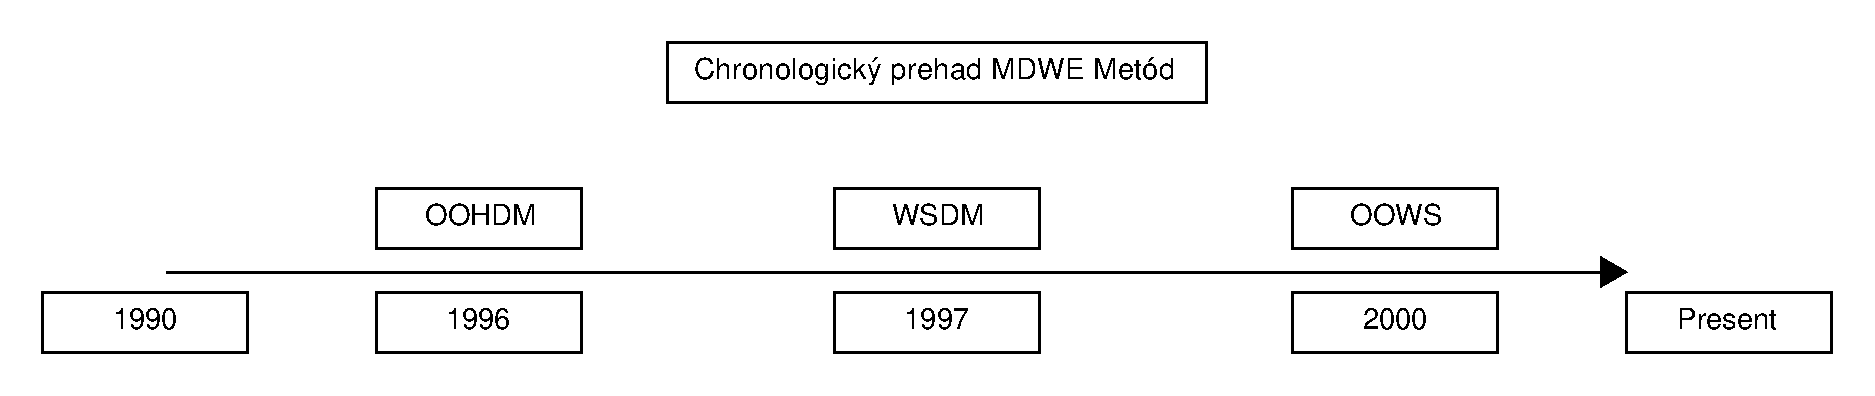
\includegraphics[scale=0.4]{./Visuals/Chronologický prehľad MDWE metód.pdf}.
\caption{Chronologický prehľad MDWE metód (upravený\cite{Valderas:MDDE}).}
\label{Prehľad}
\end{figure*}


\subsection{OOHDM: Object Oriented Hypermedia Design Model} \label{OOHDM}

OOHDM bolo vyvinuté pánmi Schwabe a Rossi v roku 1994. Bolo to jedno z prvých metodologických riešení pre vývoj webových aplikácií. OOHDM zdôrazňuje separáciu navigačných aspektov softvéru od iných aspektov, ako napríklad koncepčné aspekty a aspekty rozhrania. Ďalšie prístupy boli neskôr inšpirované touto myšlienkou separácií rôznych aspektov. "Nakoniec, je dôležité spomenúť, že OOHDM nie je uzatvorený prístup a je postupne rozširovaný a vylepšovaný."\cite{Valderas:MDDE}\\

Proces vývoja tohto prístupu je rozdelený do piatich hlavných fáz:\\
- Zhromažďovanie požiadaviek. V tejto fáze sú definovaní užívatelia, ktorí používajú webovú aplikáciu, ako aj uživateľské potreby, ktoré musí webová aplikácia podporovať.\\
- Koncepčný dizajn. Táto fáza pozostáva z koncepčnej schémy, v ktorej sú popísané statické systémové aspekty.\\
- Navigačný dizajn. V tejto fáze musí byť definovaný diagram navigačných tried a diagram navigačnej štruktúry. Prvý reprezentuje statické možnosti navigačného systému. Druhý, na druhej strane, rozširuje prvý diagram o prístupové štruktúry a navigačný kontext.\\
- Abstraktný dizajn rozhrania. Táto fáza definuje opis užívaťeľského rozhrania abstraktným spôsobom.\\
- Implementácia. V tejto fáze je webová aplikácia implementovaná. Táto implementácia je založená na predchádzajúcich modeloch.\cite{Valderas:MDDE}\\


\subsection{OOWS: Object Oriented Web Solutions} \label{OOWS}
Ďalej nasleduje novšia metóda s názvom OOWS. Síce sa nejedná o následujúcu metódu vrámci chroronolockej postupnosti, ale článok ju popisuje priamo po OOHDM metóde, pretože obidve tieto metódy majú rovnaký základ, a to objektovo-orientovaný prístup.\\ 
Táto metóda bola prvýkrát prezentovaná pánmi Joan Fons a Oscar Pastor v roku 2000. Ide o rozšírenie objektovo-orientovaného prístupu pri vývoji webových aplikácií. Narozdiel od OO-H (object-oriented hypermedia) prístupu, táto metóda je založená iba na objektovo-oriantovanej báze. "Toto robí OOWS jednu z mála MDD metód, ktoré poskytujú podporu pre automatické generovanie rozhraní webových aplikácií, ako aj plne operatívnu funkčnosť vyjadrenú z modelov."\cite{Valderas:MDDE}\\

Vývojivý proces obsiahnutý v tomto prístupe je rozdelený na tri hlavné fázy:\\
- Analýza požiadaviek. V tejto fáze sú špecifikované požiadavky webovej aplikácie pomocou modelov, ktoré sú založené na koncepte úloh (concept of task). Je dôležité poznamenať, že táto fáza bola uvedená do praxe až po pridaní rôznych rozšírení do tejto metódy.\\
- Špecifikácia systému. Táto časť pozostáva z popisu webovej aplikácie na koncepčnej úrovni. Na dosiahnutie tohto výsledku sú navrhnuté rôzne modely:
\begin{enumerate}
\item Objektový model na predpísanie statickej štruktúry webovej aplikácie
\item Funkčné a dynamické modely na predpísanie správania sa webovej aplikácie.
\item Navigačné a prezentačné modely na predpísanie používaťeľského rozhrania webovej aplikácie
\end{enumerate}
- Generácia riešení. V tejto poslednej fáze je webová aplikácia automaticky generovaná z modelov spomenutých v predchádzajúcich fázach. Na dosiahnutie tohto cieľa sú potrebné ale rôzne nástroje.\cite{Valderas:MDDE}

\subsection{WSDM: Web Site Design Method} \label{WSDM}

Nakoniec následuje posledná metóda s názvom WSDM. Táto sa od predošlých líši, mimo iného, aj v tom, že nie je založená na objektovo-orientovanom prístupe.\\
WSDM metóda bola vyvinutá pánmi De Troyer a Leune v roku 1998. Ide teda o nepatrne novšiu metódu ako OOHDM ale staršiu ako OOWS.\\
WSDM definuje webové aplikácie popisovaním požiadaviek rôznych skupín užívateľov, ktorí s ňou zaobchádzajú. Ide teda o metódu, ktorá definuje užívateľa ako centrum tohto prístupu. Je to jedna z prvých metód, ktorá prihliada na problém vysokej rôznorodosti užívateľov vo webových aplikáciách.\cite{Valderas:MDDE}\\

Vývojový proces tohto prístupu je rozdelený do piatich hlavných fáz:\\
- Špecifikácia poslania. V tejto fáze je potrebné definovať účel a predmet webovej aplikácie. Tatiež musí byť poukázané na cieľové publikum, pre kroté je daná  aplikácia vyvíjaná.\\
- Modelovanie publika. V druhej fáze sú špecifikovaný užívatelia a sú následne rozdelení do skupín. Toto je vykonané za účelom študovanie systémových požiadaviek na základe každej skupiny.\\
- Koncepčný dizajn. V tretej fáze je vytvorený diagram tried a navigačný model. Diagram tried reprezentuje statický model systému a navigačný model popisuje možnosti navigácie vo webovej aplikácii. 
- Implementačný dizajn. Počas štvrtej fázy sú definované koncepčné dizajnové modely. Tieto modely sú následne doplnené o informácie, potrebné na samotnú implementáciu. Takéto informácie sú napríklad model štruktúry stránky alebo prezentačný model.\\

\section{Porovnanie MDWE metód} \label{ina}

Hlavné porovnanie MDWE metód + tabuľky

\begin{figure*}[tbh]
\centering
\includegraphics[scale=0.4]{./Visuals/OOHDM Conceptual Model.pdf}.
\caption{Príklad koncepčného modelu pre obchod s CD (upravený\cite{Schwabe:OOHDM}).}
\label{Conceptual OOHDM Model}
\end{figure*}

\section{Popis MDA prístupu}


MDA prístup je široko využívaný softvérovými inžiniermi pri vyvíjaní webových aplikácií.\\
Častokrát, pri MDD metódach, je interakcia medzi používateľom a systémom nie presne špecifikovaná. Často je rozhranie systému generované pre rozličné platformy (stolný počítač, web, mobilný telefón..) z rovnakého modelu. Tým sa vytvára priestor pre rozličné komplikácie spojené so systémovým rozhraním. V tom prípade je nutné klásť väčší dôraz na presnejšie špecifikovanie koncepčných modelov. Preto je v tomto prípade MDA prístup veľmi zaujímavým riešením.\cite{Valverde:MDA}
MDA (Model-Driven Architecture) je prístup využívaný v modelovo založenom softvérovom vývojárstve a predstavuje viacero modelov. Tieto modely majú za úlohu vylepšiť a spresniť proces vývoja softvéru. Prvým z nich je CIM (Computation-Independent model), v preklade model nezávyslý na výpočte.  Tento model neberie ohľad na výpočtové aspekty spojené s modelovaním systému a je zameraný výlučne na požiadavky systému a jeho prostredia. Ďalším modelom je PIM (Platform-Independent Model), ktorý popisuje interakciu s danou platformou, bez toho, aby uvažoval technologické aspekty platformy. Preto nakoniec nasleduje posledný model PSM (Platform Specific Model). Tento model vychádza z predošlého modelu a už presne popisuje technologické požiadavky rôznych platfórm, na ktoré bude webová aplikácia následne implementovaná. Nakoniec je vytvorený model kódu z PSM modelu. Transformácia týchto modelov je automatická alebo polo-automatická. To záleží od MDA prostredia, ktoré ich podporuje.\cite{Pastor:MDD}

\section{Porovnanie MDWE metód vyžívajúcich MDA prístup}

Postupom rokov sa začali prejavovať slabšie stránky predošle spomenutých metód. Jedna z nich bola spomenutá v predchádzajúcej sekcii. Preto za účelom odtránenia týchto nedokonalostí sa začal využívať MDA prístup v spojení so spomenutými metódami. Tak vznikli hybridné metódy, ktoré využívajú techniky a postupy obsiahnuté v základných metódach, ale sú obohatené o postupy definované v MDA paradigme. Takýmito hybridnými metódami sú napríklad OOHDMDA, OOWS a WSDMA. Vďaka implementovaniu týchto postupov sa stávajú dané metódy efektívnejšie v oblasti vývoja webových aplikácií.\\
Ďalej budú tieto metódy bližšie špecifikované a porovnané. 

\subsection{OOHDMDA}

OOHDMDA je modelovacia metóda, ktorá kombinuje vlastnosti OOHDM metódy a prvky MDA prístupu. Jej hlavným cieľom je transformácia koncepčného modelu základnej metódy na PIM model využitím ... Ďalej nasleduje transformáca na PSM model využitím servlet-based dacoho. 

\subsection{OOWS}

\subsection{WSDMDA}

WSDMDA je MDA-založená metóda na vývoj webových aplikácií. Ako z názvu vyplýva, tak je založená na existujúcej WSDM metóde spomenutej vyššie v článku. WSDMDA zvyšuje efektivitu základnej metódy tým, že poskytuje vyššiu rýchlosť generovania komplexného kódu ako tradičná metóda. Výsledkom tejto hybridnej metódy oproti základnej je taktiež schopnosť narábať aj s dynamickou webovou aplikáciou namiesto narábania jedine so statickou. Toto je doshianuté vďaka tomu, že vrchná časť webovej stránky sa mení v závislosti od používateľských záujmov, kým druhá časť ostáva taká, aká bola definovaná webovýmm dizajnérom. Profil týchto používateľských záujmov je využívaný počas chodu webovej aplikácie, ze cieľom zobrazovania špeciálnych položiek, ktoré môžu byť využité ako promócia nového produktu alebo ako reklama špecifickej témy v danej oblasti.\\
Táto metóda prerába koncepčný model tradičnej metódy, za účelom využitia tohto modelu ako PIM model, a to vďaka pridaniu používateľského záujmového profilu. Ďalej kladie veľký dôraz na následnú transformáciu na PSM model, spresnením PIM modelu.\cite{Mukhtar:WSDMDA}

\section{Zhrnutie}

Tu napíšem zhrnutie

%\section{Bibliografia}





%\acknowledgement{Ak niekomu chcete poďakovať\ldots}


% týmto sa generuje zoznam literatúry z obsahu súboru literatura.bib podľa toho, na čo sa v článku odkazujete
\bibliography{literatura}
\bibliographystyle{plain} % prípadne alpha, abbrv alebo hociktorý iný
\end{document}
